\documentclass[a4paper,12pt]{ctexart}

\usepackage{geometry}
\geometry{left=2.5cm,right=2.5cm,top=3cm,bottom=3cm}
\usepackage{graphicx}
\usepackage{booktabs}
\usepackage{longtable}
\usepackage{listings}
\usepackage{xcolor}
\usepackage{amsmath, amssymb}
\usepackage{hyperref}
\usepackage[normalem]{ulem}
\usepackage{listings}
\usepackage{subcaption}


\setlength{\parskip}{0.75em}

\newcommand{\uText}[2][3cm]{\uline{\makebox[#1][c]{#2}}}

\hypersetup{
    colorlinks=true,
    linkcolor=blue,
    citecolor=blue,
    urlcolor=blue
}

\lstset{
    basicstyle=\ttfamily\small,
    numbers=left,
    numberstyle=\tiny,
    keywordstyle=\color{blue},
    commentstyle=\color{gray},
    stringstyle=\color{red},
    frame=single,
    breaklines=true,
    showstringspaces=false
}

\begin{document}

\begin{titlepage}
    \centering
    \vspace*{3cm}
    {\Huge\bf 系统开发工具基础实验报告\\[1.5cm]}
    {\Large\it 实验内容:\uText[4cm]{实验四}\\[0.5cm]}
    {\Large\it 姓名:\uText[4cm]{张家宜} \quad 学号:\uText[5cm]{2024020013045}\\[0.5cm]}
    {\Large\it 日期:\today\\[1.5cm]}
    \vfill
    \normalsize
    \vspace*{1cm}
\end{titlepage}

% 目录
\tableofcontents
\newpage

    
\section{练习内容}

\subsection{调试及性能分析}
\subsubsection{打印调试法与日志}

调试代码可以在程序中直接打印出来语句,还可以使用日志

日志可以支持严重等级(例如 INFO, DEBUG, WARN, ERROR 等),可以根据需要过滤日志

在终端可以使用ANSI escape code来打印出来颜色,让日志更加可读

执行 \verb|echo -e "\e[38;2;255;0;0mThis is red\e[0m"| 会打印红色的字符串

\subsubsection{第三方日志系统}
大多数的程序都会将日志保存在系统中的某个地方。对于 UNIX 系统程序的日志通常存放在 /var/log

Linux系统中可以使用systemd

systemd 会将日志以某种特殊格式存放于 /var/log/journal,可以使用 journalctl 命令显示这些消息

\begin{lstlisting}
$ logger "Hello Logs"
$ journalctl --since "1m ago" | grep Hello
Sep 23 15:44:09 rott[1268]: Hello Logs
\end{lstlisting}

\subsubsection{调试器}
很多编程语言都有自己的调试器,Python 的调试器是 pdb

\begin{tabular}{|l|p{10cm}|}
\hline
\textbf{命令} & \textbf{说明} \\
\hline
l (list) & 显示当前行附近的 11 行或继续执行之前的显示 \\
\hline
s (step) & 执行当前行,并在第一个可能的地方停止 \\
\hline
n (next) & 继续执行直到当前函数的下一条语句或者 return 语句 \\
\hline
b (break) & 设置断点(基于传入的参数) \\
\hline
p (print) & 在当前上下文对表达式求值并打印结果。还有一个命令是 pp,它使用 pprint 打印 \\
\hline
r (return) & 继续执行直到当前函数返回 \\
\hline
q (quit) & 退出调试器 \\
\hline
\end{tabular}

还可以使用ipdb(增强的pdb)让调试过程中有 tab 补全、语法高亮、更好的回溯和更好的内省

\subsubsection{专门工具}
\begin{enumerate}
  \item 在 Linux 中可以使用 \texttt{strace}  
    \begin{lstlisting}
    # 使用 strace 来显示 ls 执行时,对 stat 系统调用进行追踪
    $ sudo strace -e lstat ls -l > /dev/null
    +++ exited with 0 +++
    \end{lstlisting}

  \item 对于网络数据包分析可以使用 \texttt{tcpdump} 和 \texttt{Wireshark}

  \item 对于 Web 开发,可以使用 Chrome/Firefox 的开发者工具
\end{enumerate}

\subsubsection{pyflaskes}
我们可以使用一些工具对代码进行静态分析,找出一些语法错误等等

Python可以使用 pyflakes 分析代码

\begin{lstlisting}
$ cat b.py
import time

def foo():
    return 42

for foo in range(5):
    print(foo)
bar = 1
bar *= 0.2
time.sleep(60)
print(baz)
$ pyflakes3 b.py
b.py:6:5: redefinition of unused 'foo' from line 3
b.py:11:7: undefined name 'baz'
\end{lstlisting}

\subsubsection{shellcheck}

可以使用shellcheck下面的脚本进行检查

\begin{lstlisting}
#!/bin/sh
## Example: a typical script with several problems
for f in $(ls *.m3u)
do
  grep -qi hq.*mp3 $f \
    && echo -e 'Playlist $f contains a HQ file in mp3 format'
done
\end{lstlisting}

输出:
\begin{lstlisting}
$ shellcheck a.sh

In a.sh line 1:
u#!/bin/sh
^-- SC2148 (error): Tips depend on target shell and yours is unknown. Add a shebang or a 'shell' directive.


In a.sh line 3:
for f in $(ls *.m3u)
         ^---------^ SC2045 (error): Iterating over ls output is fragile. Use globs.
              ^-- SC2035 (info): Use ./*glob* or -- *glob* so names with dashes won't become options.


In a.sh line 5:
  grep -qi hq.*mp3 $f \
           ^-----^ SC2062 (warning): Quote the grep pattern so the shell won't interpret it.
                   ^-- SC2086 (info): Double quote to prevent globbing and word splitting.

Did you mean:
  grep -qi hq.*mp3 "$f" \


In a.sh line 6:
    && echo -e 'Playlist $f contains a HQ file in mp3 format'
               ^-- SC2016 (info): Expressions don't expand in single quotes, use double quotes for that.

For more information:
  https://www.shellcheck.net/wiki/SC2045 -- Iterating over ls output is fragi...
  https://www.shellcheck.net/wiki/SC2148 -- Tips depend on target shell and y...
  https://www.shellcheck.net/wiki/SC2062 -- Quote the grep pattern so the she...
\end{lstlisting}

\subsubsection{性能分析可视化}

使用分析器来分析真实的程序时,可以使用一些工具可视化分析器输出结果

在 Python 中可以使用 pycallgraph 来生成这些图片
\begin{figure}[htbp]
  \centering
  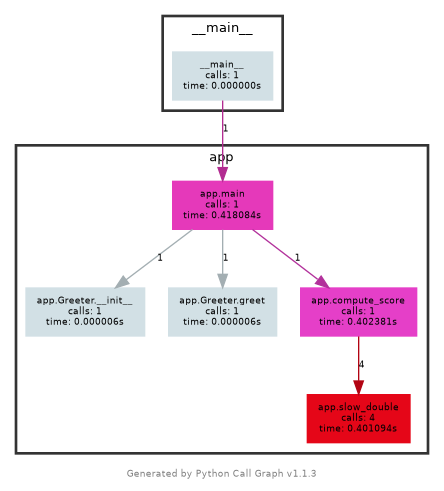
\includegraphics[width=0.5\linewidth]{callgraph.png}
  \caption{PyCallGraph 生成的调用关系图示例}
  \label{fig:py-callgraph}
\end{figure}


\subsubsection{htop 资源监控}
使用 \texttt{htop} 可以实时查看节点的进程情况、CPU 和内存占用率,如图 \ref{fig:htop} 所示。
\begin{figure}[htbp]
  \centering
  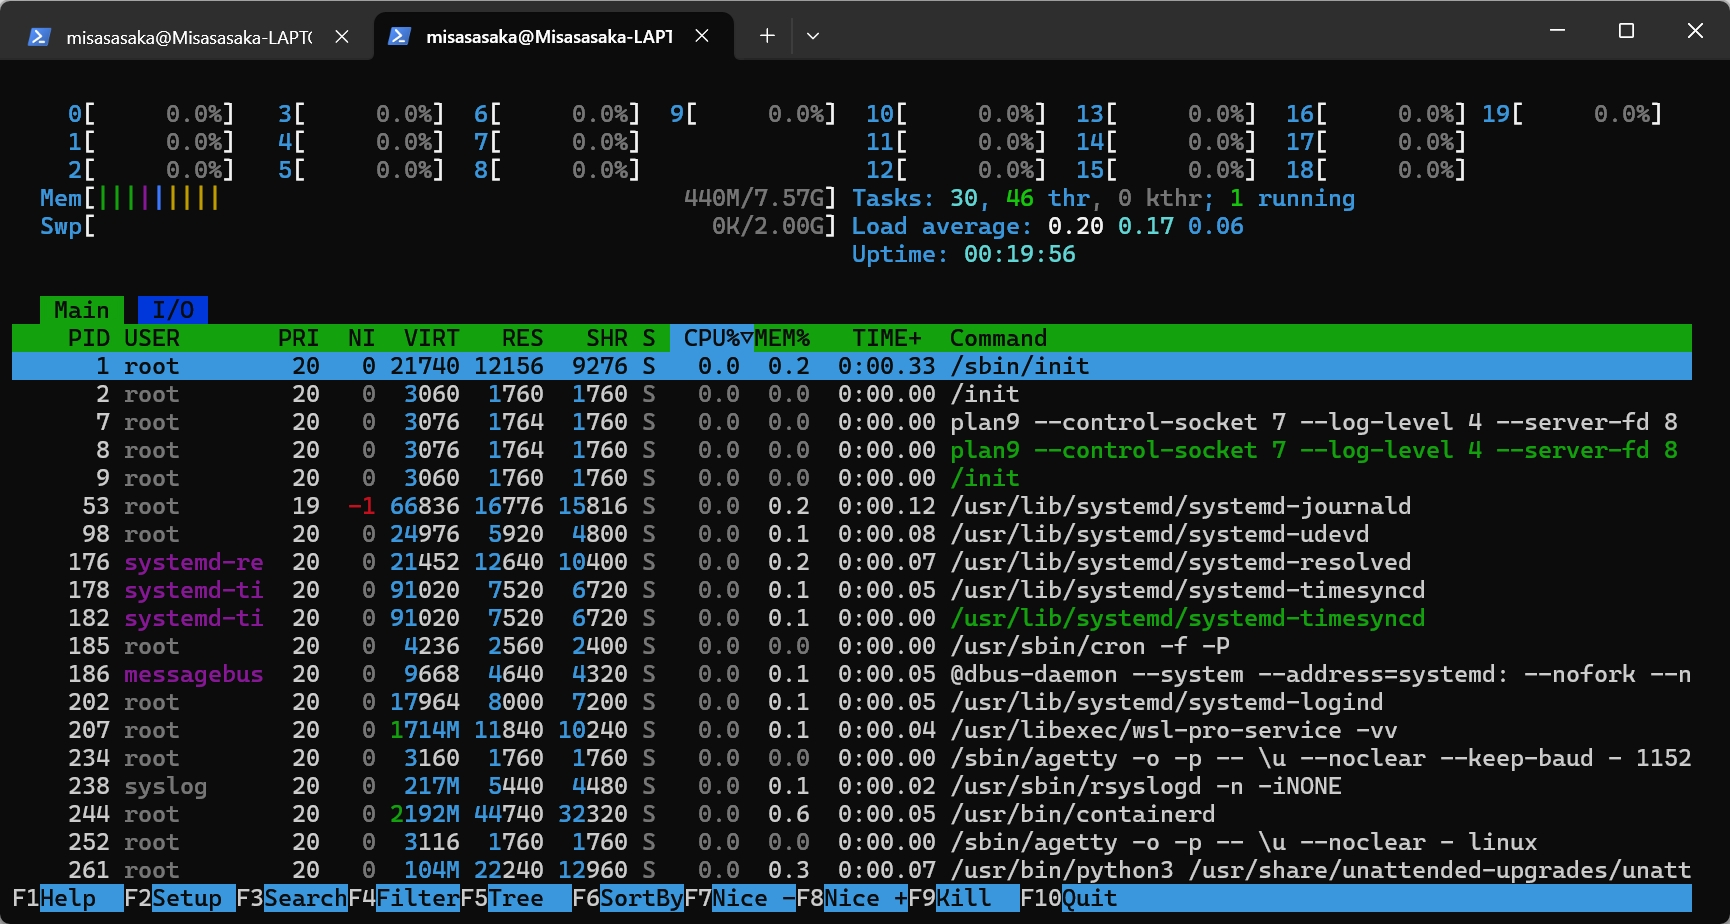
\includegraphics[width=0.9\linewidth]{htop.jpg}
  \caption{htop 进程与 CPU/内存占用}
  \label{fig:htop}
\end{figure}

\subsubsection{df 磁盘占用}
通过 \texttt{df -h} 命令可以监控磁盘空间使用情况,帮助判断存储是否接近上限,如图 \ref{fig:df} 所示。
\begin{figure}[htbp]
  \centering
  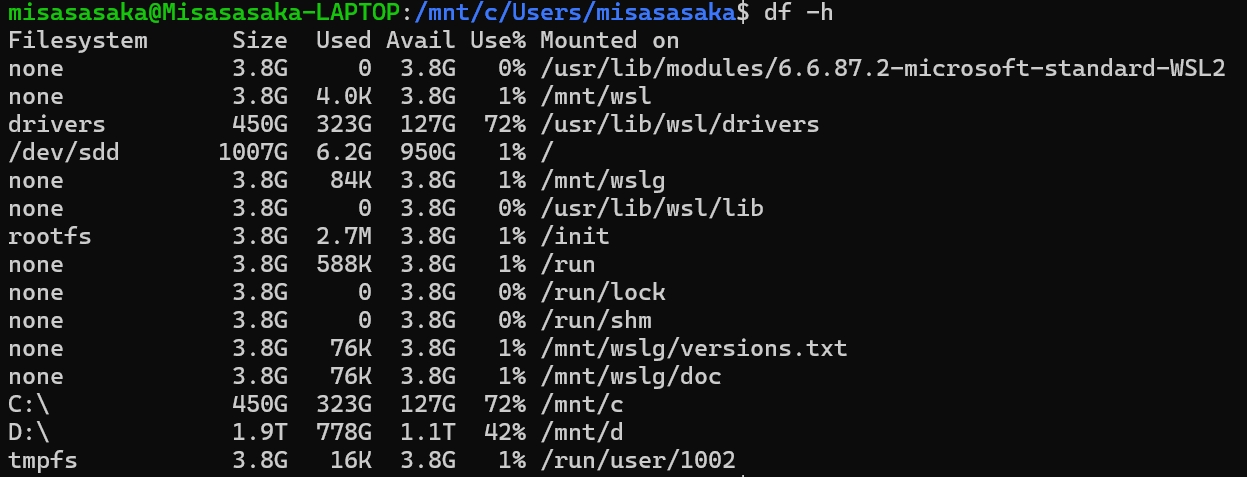
\includegraphics[width=0.9\linewidth]{df.jpg}
  \caption{df 磁盘占用}
  \label{fig:df}
\end{figure}


\newpage

\subsection{元编程}

\subsubsection{构建系统}
make 是最常用的构建系统之一

以下是一个示例

\begin{lstlisting}
$ ls
Makefile  apple.png
$ cat Makefile
PNG_FILES := $(wildcard *.png)
JPG_FILES := $(PNG_FILES:.png=.jpg)

all: $(JPG_FILES)

%.jpg: %.png
        convert $< $@

misasasaka@Misasasaka-$ make
convert apple.png apple.jpg
$ ls
Makefile  apple.jpg  apple.png
\end{lstlisting}

\subsubsection{依赖管理}

在软件项目中,依赖可以是其他程序、系统包或语言库,通常通过软件仓库(如 Ubuntu 的 \texttt{apt}、Ruby 的 RubyGems、Python 的 PyPi、Arch 的 AUR)统一获取与安装。为了保证软件构建的稳定性,依赖项目会使用\textbf{版本控制},常见的格式为语义版本号 \texttt{主.次.补丁}:补丁号表示向后兼容的修复,次版本号表示向后兼容的新功能,主版本号表示不兼容的重大改动。例如 Python 2 与 Python 3 的不兼容便体现了主版本号的重要性。依赖管理中还涉及\textbf{锁文件}(lock files),它记录当前依赖的具体版本,以实现可复现构建并防止自动升级;而\textbf{vendoring} 则是极端的依赖锁定方式,将依赖代码直接拷贝进项目,便于修改和完全控制,但需手动同步上游更新。

\subsubsection{持续集成系统}

持续集成(Continuous Integration, CI)指在代码发生变动时自动执行一系列任务,如测试、构建、发布等。常见的 CI 工具有 Travis CI、Azure Pipelines 和 GitHub Actions,其核心是在仓库中添加配置文件以描述触发条件和执行步骤:例如代码提交后自动运行测试套件、检查代码风格并生成构建结果。CI 服务会启动虚拟机执行规则并记录结果,可设置通知或在仓库主页显示测试徽标。GitHub Pages 即是典型案例,每次 \texttt{master} 更新会自动构建站点。\\

测试体系:测试套件(Test suite)是全部测试的集合;单元测试(Unit test)关注单个功能的正确性;集成测试(Integration test)验证系统各组件的协同工作;回归测试(Regression test)确保已修复的 bug 不会重现;模拟(Mocking)通过假实现屏蔽外部依赖,如模拟网络或硬盘,以专注被测功能。


\subsection{PyTorch}

\subsubsection{安装}
\begin{itemize}
  \item 使用 \textbf{conda} 或 \textbf{pip} 安装:
  \begin{verbatim}
  conda install pytorch torchvision torchaudio -c pytorch
  \end{verbatim}
  \item 检查 GPU 是否可用:
  \begin{verbatim}
  torch.cuda.is_available()
  \end{verbatim}
\end{itemize}


\subsubsection{Tensor(张量)}
\begin{itemize}
  \item PyTorch 的核心数据结构,像 NumPy 的数组,但可以在 GPU 上计算。
  \item 创建方法:
  \begin{verbatim}
  torch.tensor()
  torch.zeros()
  torch.rand()
  \end{verbatim}
  \item 常用操作:索引、切片、加减乘除、\texttt{view} 或 \texttt{reshape} 改变形状。
\end{itemize}

\subsubsection{自动求导}
\begin{itemize}
  \item 创建张量时加 \texttt{requires\_grad=True} 会自动记录计算过程。
  \item 调用 \texttt{loss.backward()} 自动计算梯度,结果保存在 \texttt{.grad} 中。
\end{itemize}

\subsubsection{网络模块}
\begin{itemize}
  \item \texttt{torch.nn} 提供神经网络层和激活函数,如 \texttt{nn.Linear}、\texttt{nn.ReLU}。
  \item 自定义模型:继承 \texttt{nn.Module} 并编写 \texttt{forward()} 定义前向传播。
\end{itemize}

\subsubsection{训练流程}
\begin{itemize}
  \item 选择优化器,例如 \texttt{torch.optim.SGD} 或 \texttt{Adam}。
  \item 训练步骤:
  \begin{enumerate}
    \item 前向计算输出
    \item 计算损失
    \item \texttt{loss.backward()} 反向传播
    \item \texttt{optimizer.step()} 更新参数
    \item \texttt{optimizer.zero\_grad()} 清空梯度
  \end{enumerate}
\end{itemize}

\subsubsection{数据处理}
\begin{itemize}
  \item \texttt{torchvision.datasets} 提供常见数据集(如 MNIST、CIFAR)。
  \item 使用 \texttt{DataLoader} 可批量读取并打乱数据。
\end{itemize}

\subsubsection{GPU 使用}
\begin{itemize}
  \item 将模型或数据放到 GPU:
  \begin{verbatim}
  model.to('cuda')
  tensor.to('cuda')
  \end{verbatim}
  \item 确保模型和输入在同一设备上。
\end{itemize}


\subsubsection{实例}

这里我选的是 文本情感分析项目

使用的\href{https://ai.stanford.edu/~amaas/data/sentiment}{IMDb电影评论数据集}。


源码可以在github仓库中查看

\begin{figure}[htbp]
  \centering
  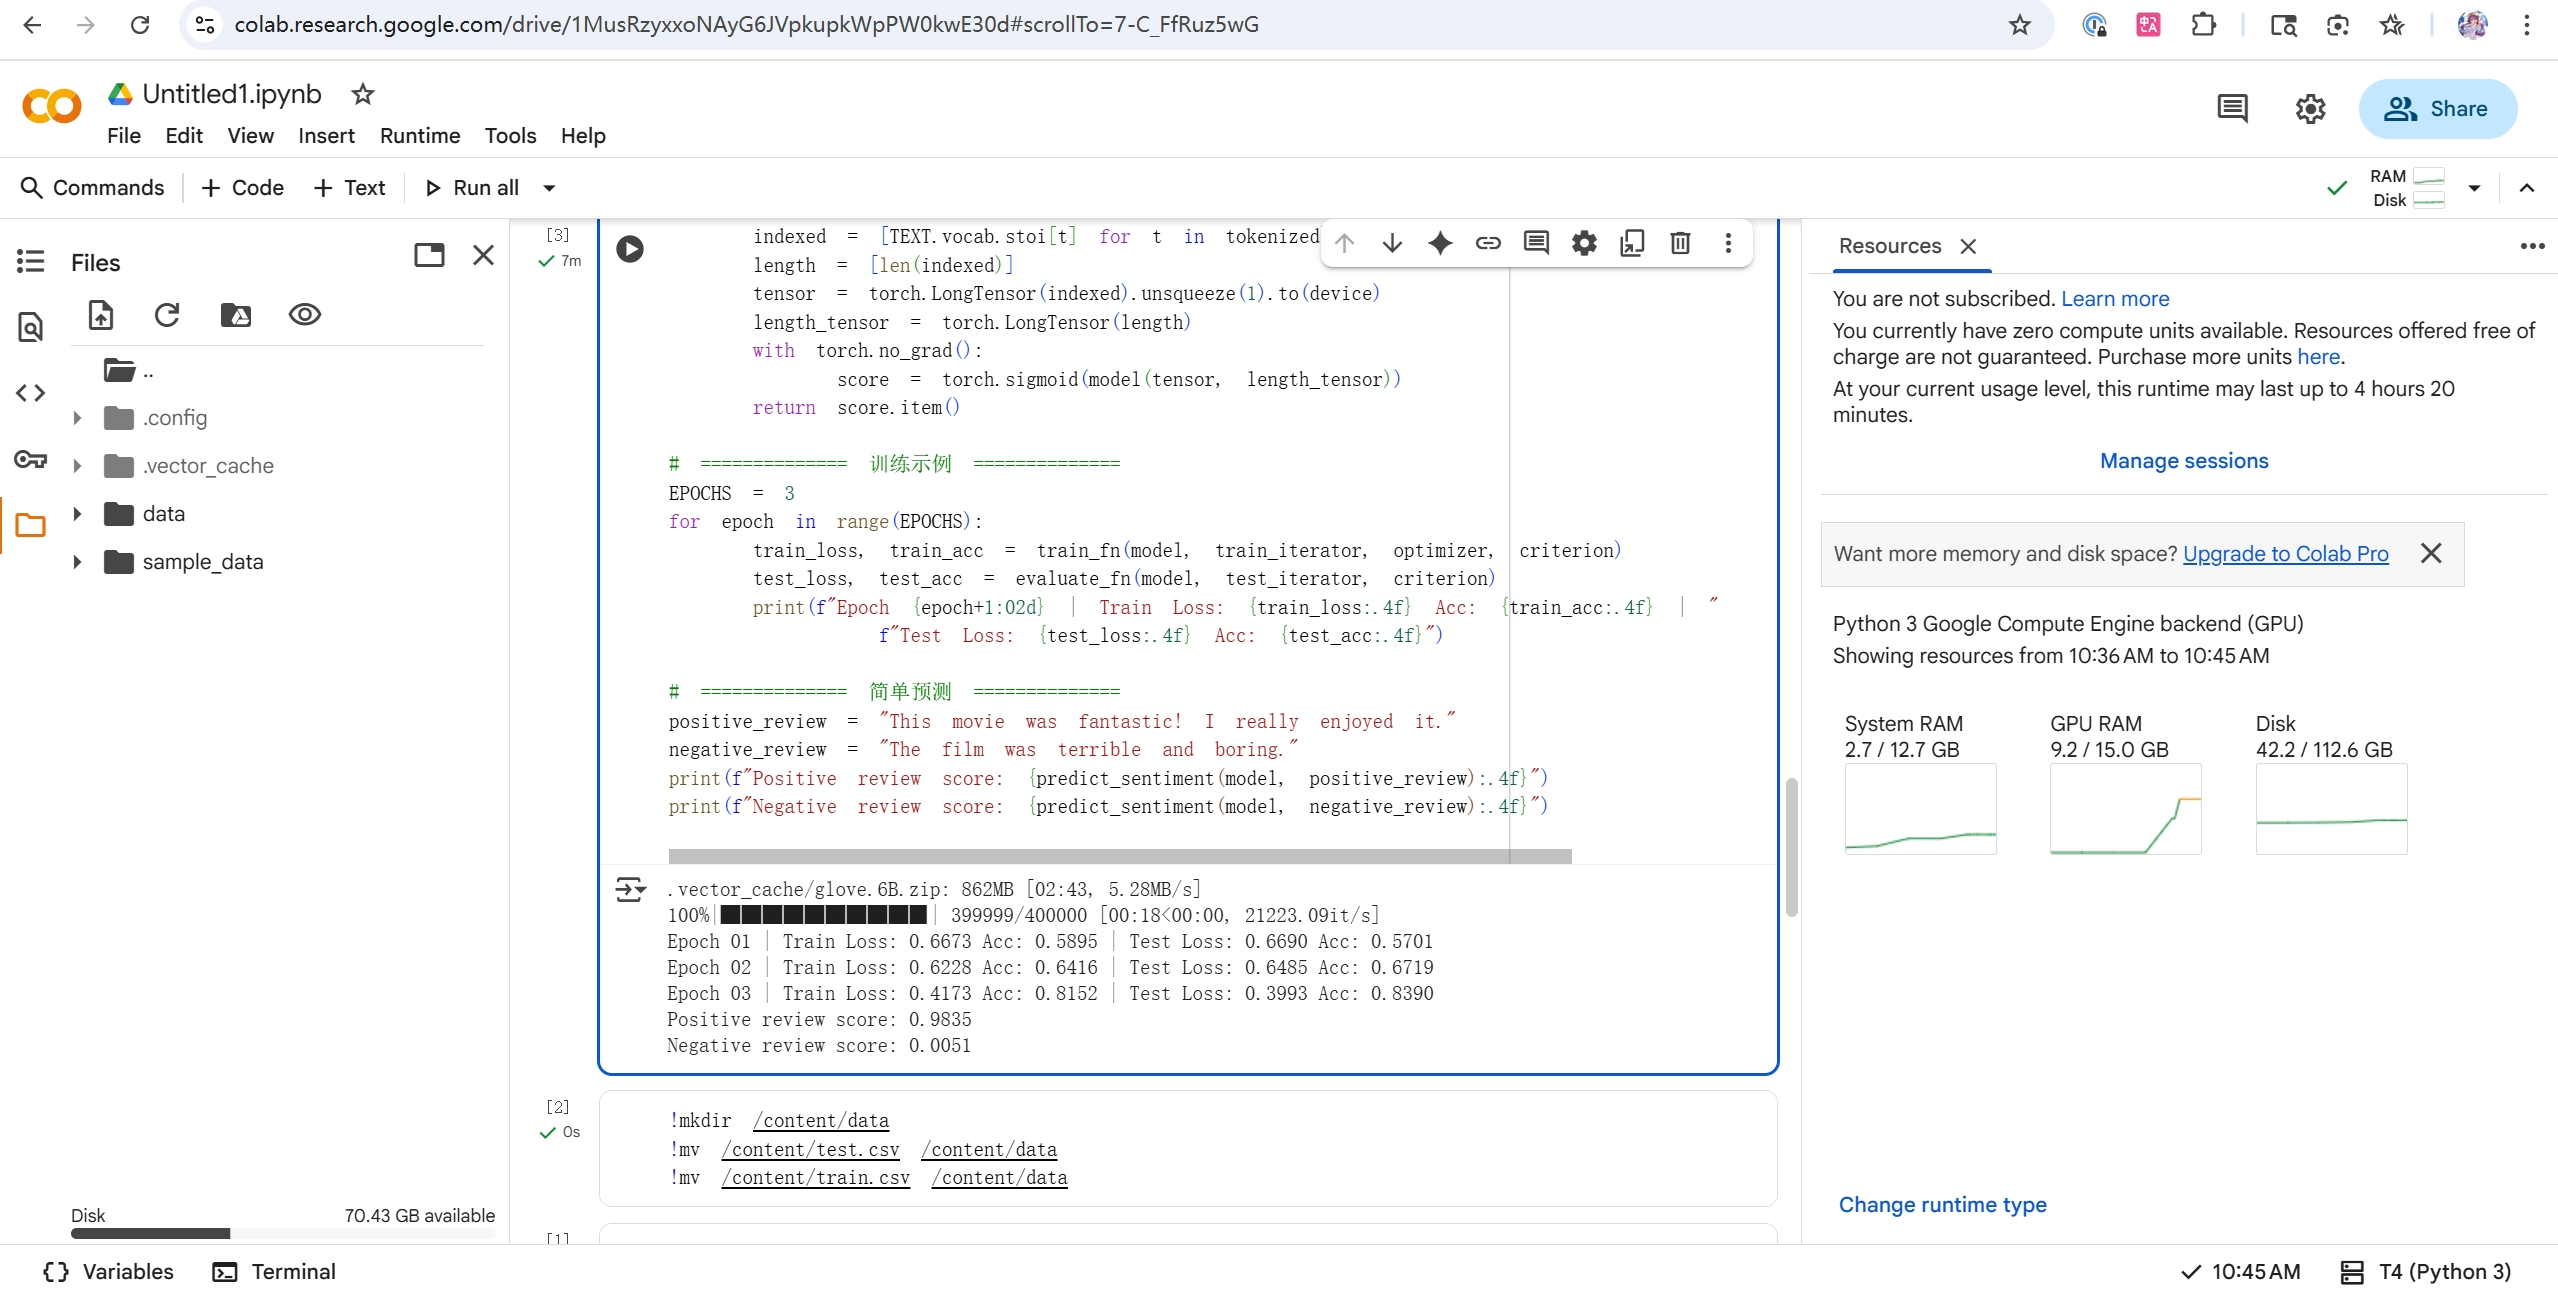
\includegraphics[width=0.6\textwidth]{pytorch.jpg}
  \caption{运行结果}
  \label{fig:pytorch}
\end{figure}

预测的结果无误


\newpage

\section{解题感悟}
不同层级的工具能在不同场景下提供精准的排查手段,结合日志系统与 ANSI 颜色输出,可以让排错过程更直观高效,也更加符合实际工程需求。

\vspace{14pt}

在性能分析与可视化部分,通过 \texttt{pycallgraph} 等工具生成调用关系图,不仅能直观看到程序执行的关键路径,也能帮助发现潜在的性能瓶颈。

\vspace{14pt}

元编程与自动化构建环节,则让我感受到工程化的重要性。从 \texttt{make} 构建系统到依赖管理与持续集成,每一步都体现了软件开发中“可复现”和“自动化”的核心理念。

\vspace{14pt}

PyTorch 是流行的机器学习平台,这次实践也让我了解了如何训练一个模型,如何去使用训练好的模型。

\newpage

\begin{thebibliography}{9}
\bibitem{missing-semester} Missing Semester 中文版,\url{https://missing-semester-cn.github.io/}
\bibitem{runoob} Pytorch教程,\url{https://www.runoob.com/pytorch/pytorch-tutorial.html}
\end{thebibliography}

\section*{GitHub 链接}
\begin{center}
\href{https://github.com/Misasasasasaka/report/tree/main/P4}{https://github.com/Misasasasasaka/report/tree/main/P4}
\end{center}

\end{document}
